% Options for packages loaded elsewhere
\PassOptionsToPackage{unicode}{hyperref}
\PassOptionsToPackage{hyphens}{url}
%
\documentclass[
  letterpaper,
  ignorenonframetext,
  aspectratio=43,
  handout,
  12pt]{beamer}
\usepackage{pgfpages}
\setbeamertemplate{caption}[numbered]
\setbeamertemplate{caption label separator}{: }
\setbeamercolor{caption name}{fg=normal text.fg}
\beamertemplatenavigationsymbolsempty
% Prevent slide breaks in the middle of a paragraph
\widowpenalties 1 10000
\raggedbottom
\setbeamertemplate{part page}{
  \centering
  \begin{beamercolorbox}[sep=16pt,center]{part title}
    \usebeamerfont{part title}\insertpart\par
  \end{beamercolorbox}
}
\setbeamertemplate{section page}{
  \centering
  \begin{beamercolorbox}[sep=12pt,center]{part title}
    \usebeamerfont{section title}\insertsection\par
  \end{beamercolorbox}
}
\setbeamertemplate{subsection page}{
  \centering
  \begin{beamercolorbox}[sep=8pt,center]{part title}
    \usebeamerfont{subsection title}\insertsubsection\par
  \end{beamercolorbox}
}
\AtBeginPart{
  \frame{\partpage}
}
\AtBeginSection{
  \ifbibliography
  \else
    \frame{\sectionpage}
  \fi
}
\AtBeginSubsection{
  \frame{\subsectionpage}
}
\usepackage{amsmath,amssymb}
\usepackage{lmodern}
\usepackage{ifxetex,ifluatex}
\ifnum 0\ifxetex 1\fi\ifluatex 1\fi=0 % if pdftex
  \usepackage[T1]{fontenc}
  \usepackage[utf8]{inputenc}
  \usepackage{textcomp} % provide euro and other symbols
\else % if luatex or xetex
  \usepackage{unicode-math}
  \defaultfontfeatures{Scale=MatchLowercase}
  \defaultfontfeatures[\rmfamily]{Ligatures=TeX,Scale=1}
\fi
\usetheme[]{metropolis}
% Use upquote if available, for straight quotes in verbatim environments
\IfFileExists{upquote.sty}{\usepackage{upquote}}{}
\IfFileExists{microtype.sty}{% use microtype if available
  \usepackage[]{microtype}
  \UseMicrotypeSet[protrusion]{basicmath} % disable protrusion for tt fonts
}{}
\makeatletter
\@ifundefined{KOMAClassName}{% if non-KOMA class
  \IfFileExists{parskip.sty}{%
    \usepackage{parskip}
  }{% else
    \setlength{\parindent}{0pt}
    \setlength{\parskip}{6pt plus 2pt minus 1pt}}
}{% if KOMA class
  \KOMAoptions{parskip=half}}
\makeatother
\usepackage{xcolor}
\IfFileExists{xurl.sty}{\usepackage{xurl}}{} % add URL line breaks if available
\IfFileExists{bookmark.sty}{\usepackage{bookmark}}{\usepackage{hyperref}}
\hypersetup{
  hidelinks,
  pdfcreator={LaTeX via pandoc}}
\urlstyle{same} % disable monospaced font for URLs
\newif\ifbibliography
\usepackage{graphicx}
\makeatletter
\def\maxwidth{\ifdim\Gin@nat@width>\linewidth\linewidth\else\Gin@nat@width\fi}
\def\maxheight{\ifdim\Gin@nat@height>\textheight\textheight\else\Gin@nat@height\fi}
\makeatother
% Scale images if necessary, so that they will not overflow the page
% margins by default, and it is still possible to overwrite the defaults
% using explicit options in \includegraphics[width, height, ...]{}
\setkeys{Gin}{width=\maxwidth,height=\maxheight,keepaspectratio}
% Set default figure placement to htbp
\makeatletter
\def\fps@figure{htbp}
\makeatother
% Make links footnotes instead of hotlinks:
\DeclareRobustCommand{\href}[2]{#2\footnote{\url{#1}}}
\setlength{\emergencystretch}{3em} % prevent overfull lines
\providecommand{\tightlist}{%
  \setlength{\itemsep}{0pt}\setlength{\parskip}{0pt}}
\setcounter{secnumdepth}{-\maxdimen} % remove section numbering
\usepackage{pgfpages}
\pgfpagesuselayout{2 on 1}
\providecommand{\tightlist}{%
\setlength{\itemsep}{0pt}\setlength{\parskip}{0pt}}
\makeatletter
\makeatother
\let\Oldincludegraphics\includegraphics
\renewcommand{\includegraphics}[2][]{\Oldincludegraphics[width=\textwidth,height=0.7\textheight,keepaspectratio]{#2}}
\ifluatex
  \usepackage{selnolig}  % disable illegal ligatures
\fi

\author{}
\date{}

\begin{document}

\begin{frame}{AE 737: Mechanics of Damage Tolerance}
\protect\hypertarget{ae-737-mechanics-of-damage-tolerance}{}
Lecture 11 - Multiple Site Damage, Mixed-Mode Fracture

Dr.~Nicholas Smith

Wichita State University, Department of Aerospace Engineering

8 March, 2021
\end{frame}

\begin{frame}{schedule}
\protect\hypertarget{schedule}{}
\begin{itemize}
\tightlist
\item
  8 Mar - Multiple Site Damage
\item
  10 Mar - Mixed-Mode Fracture
\item
  12 Mar - HW5 Due, HW4 Self-grade due
\item
  15 Mar - Exam 1 Review
\item
  17 Mar - Exam 1
\item
  19 Mar - HW5 Self-grade due
\end{itemize}
\end{frame}

\begin{frame}{outline}
\protect\hypertarget{outline}{}
\begin{itemize}
\tightlist
\item
  multiple site damage
\item
  mixed mode fracture
\end{itemize}
\end{frame}

\hypertarget{multiple-site-damage}{%
\section{multiple site damage}\label{multiple-site-damage}}

\begin{frame}{multiple site damage}
\protect\hypertarget{multiple-site-damage-1}{}
\begin{itemize}
\tightlist
\item
  Often damage can accumulate among multiple sources
\item
  This is very common when there are a series of holes, each can develop
  cracks with a potential to link up
\item
  ``link up'' occurs when the plastic zones between two adjacent cracks
  touch
\end{itemize}
\end{frame}

\begin{frame}{linkup}
\protect\hypertarget{linkup}{}
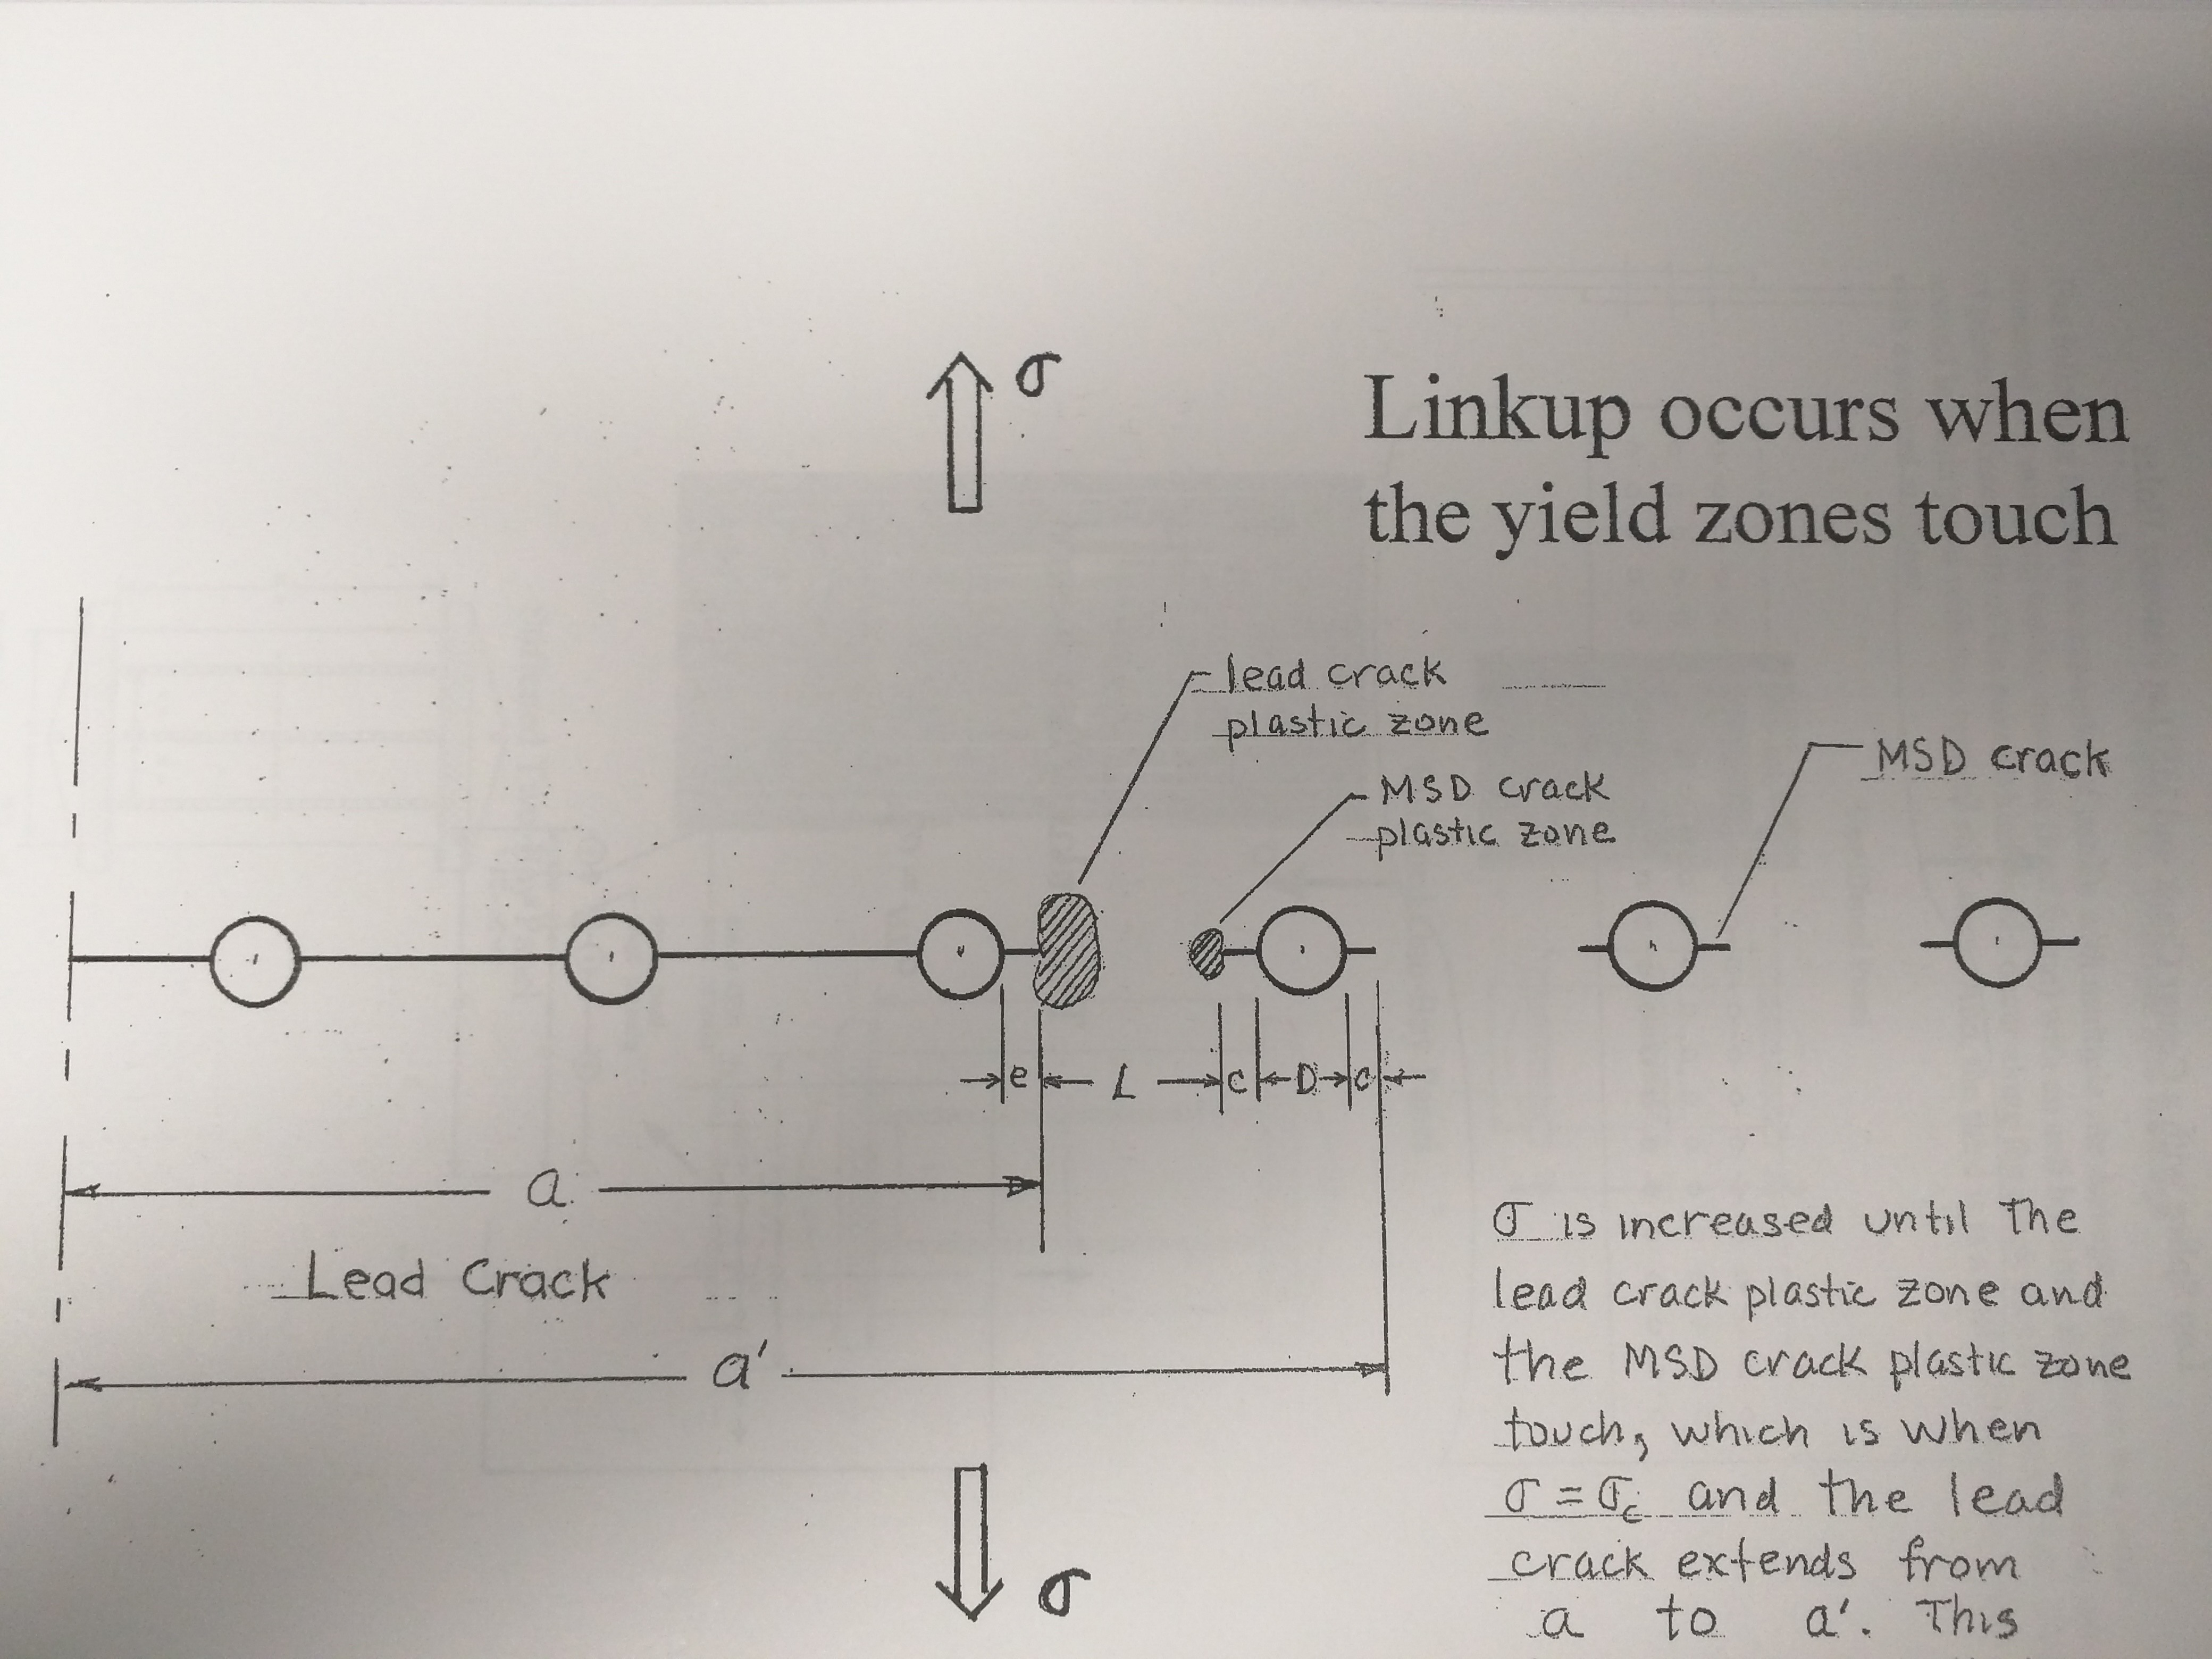
\includegraphics{../images/msd.jpg}
\end{frame}

\begin{frame}{linkup equation}
\protect\hypertarget{linkup-equation}{}
\begin{itemize}
\tightlist
\item
  We know that
\end{itemize}

\[R_p = \frac{1}{2\pi}\left(\frac{K_{Ia}}{\sigma_{YS}}\right)^2\]

\[r_p = \frac{1}{2\pi}\left(\frac{K_{Il}}{\sigma_{YS}}\right)^2\]

\begin{itemize}
\tightlist
\item
  Where we define the stress intensity factors at a and L as
\end{itemize}

\[K_{Ia} = \sigma \sqrt{\pi a} \beta_a\]

\[K_{Il} = \sigma \sqrt{\pi l} \beta_l\]
\end{frame}

\begin{frame}{linkup equation}
\protect\hypertarget{linkup-equation-1}{}
\begin{itemize}
\tightlist
\item
  Since fast cracking occurs when \(R_p + r_p = L\) we solve for the
  condition where \(R_p + r_p < L\)
\item
\end{itemize}

\[\begin{aligned}
  \frac{1}{2\pi}\left(\frac{K_{Ia}}{\sigma_{YS}}\right)^2 + \frac{1}{2\pi}\left(\frac{K_{Il}}{\sigma_{YS}}\right)^2 &&lt; L\\
  \frac{1}{2\pi\sigma_{YS}^2} \left[K_{Ia}^2 + K_{Il}^2\right] &&lt; L
\end{aligned}\]
\end{frame}

\begin{frame}{linkup equation}
\protect\hypertarget{linkup-equation-2}{}
\[\begin{aligned}
  \frac{1}{2\pi\sigma_{YS}^2} \left[\sigma^2 \pi a \beta_a^2 + \sigma^2 \pi l \beta_l^2\right] &&lt; L \\
  \frac{\sigma^2}{2\sigma_{YS}^2} \left[a \beta_a^2 + l \beta_l^2\right] &&lt; L \\
          \sigma_c &= \sigma_{YS}\sqrt{\frac{2L}{a \beta_a^2 + l \beta_l^2}}
\end{aligned}\]
\end{frame}

\begin{frame}{example}
\protect\hypertarget{example}{}
worked link-up example \href{../examples/Link-Up.html}{here}
\end{frame}

\begin{frame}{modified linkup equations}
\protect\hypertarget{modified-linkup-equations}{}
\begin{itemize}
\tightlist
\item
  We see that for a brittle material (with a small plastic zone) we
  predict no effect of ``link-up''
\item
  This does not agree with test data
\item
  Even the 2024 predictions don't agree well with test data
\item
  WSU used some empirical parameters to modify the linkup equations and
  better predict residual strength when multiple site damage is present
\end{itemize}
\end{frame}

\begin{frame}{modified 2024}
\protect\hypertarget{modified-2024}{}
\begin{itemize}
\tightlist
\item
  For 2024-T3 we use the following procedure
\item
  First find \(\sigma_c\) from the unmodified equation
\end{itemize}

\[\sigma_{c,mod} = \frac{\sigma_c}{A_1 \ln (L) + A_2}\]

\begin{itemize}
\tightlist
\item
  Where \emph{A}1 = 0.3065 and \emph{A}2 = 1.3123 for A-basis yield
  strength and \emph{A}1 = 0.3054 and \emph{A}2 = 1.3502 for B-basis
  yield strength
\item
  The same equation can also be used for 2524 with \emph{A}1 = 0.1905,
  \emph{A}2 = 0.9683 for A-basis yield and \emph{A}1 = 0.2024, \emph{A}2
  = 1.0719 for B-basis yield
\end{itemize}
\end{frame}

\begin{frame}{modified 7075}
\protect\hypertarget{modified-7075}{}
\begin{itemize}
\tightlist
\item
  A similar modification was made for 7075
\end{itemize}

\[\sigma_{c,mod} = \frac{\sigma_c}{B_1 + B_2 L}\]

\begin{itemize}
\tightlist
\item
  Where \emph{B}1 = 1.377, \emph{B}2 = 1.042 for A-basis yield strength
  and \emph{B}1 = 1.417, \emph{B}2 = 1.073 for B-basis yield strength
\end{itemize}
\end{frame}

\begin{frame}{modified 7075}
\protect\hypertarget{modified-7075-1}{}
\begin{itemize}
\tightlist
\item
  However, since general fracture had a closer prediction to real
  failure than the linkup equation, it may make more sense to modify the
  brittle fracture equation
\end{itemize}

\[\sigma_{c,mod} = \frac{K_c}{\sqrt{\pi a} (0.856 - 0.496 \ln(L))}\]
\end{frame}

\hypertarget{mixed-mode-fracture}{%
\section{mixed mode fracture}\label{mixed-mode-fracture}}

\begin{frame}{mixed-mode fracture}
\protect\hypertarget{mixed-mode-fracture-1}{}
\begin{itemize}
\tightlist
\item
  Most cracks are primarily Mode I, but sometimes Mode II can also have
  an effect
\item
  We can look at the combined stress field for Mode I and Mode II
\item
  Recall the stress field near the crack tip
\end{itemize}
\end{frame}

\begin{frame}{stress field}
\protect\hypertarget{stress-field}{}
\[\begin{aligned}
  \sigma_x &= \frac{K_I}{\sqrt{2\pi r}} \cos \frac{\theta}{2} \left(1-\sin \frac{\theta}{2}\sin \frac{3\theta}{2}\right)\\
  \sigma_y &= \frac{K_I}{\sqrt{2\pi r}} \cos \frac{\theta}{2} \left(1+\sin \frac{\theta}{2}\sin \frac{3\theta}{2}\right)\\
  \tau_{xy} &= \frac{K_I}{\sqrt{2\pi r}} \sin \frac{\theta}{2} \cos \frac{\theta}{2}\cos \frac{3\theta}{2}
\end{aligned}\]
\end{frame}

\begin{frame}{mixed-mode fracture}
\protect\hypertarget{mixed-mode-fracture-2}{}
\begin{itemize}
\tightlist
\item
  For Mode II we have
\end{itemize}

\[\begin{aligned}
  \sigma_x &= \frac{-K_{II}}{\sqrt{2\pi r}} \sin \frac{\theta}{2} \left(2+\cos \frac{\theta}{2}\cos \frac{3\theta}{2}\right)\\
  \sigma_y &= \frac{K_{II}}{\sqrt{2\pi r}} \sin \frac{\theta}{2} \cos \frac{\theta}{2}\cos \frac{3\theta}{2}\\
  \tau_{xy} &= \frac{K_{II}}{\sqrt{2\pi r}} \cos \frac{\theta}{2} \left(1-\sin \frac{\theta}{2}\sin \frac{3\theta}{2}\right)
\end{aligned}\]
\end{frame}

\begin{frame}{polar coordinates}
\protect\hypertarget{polar-coordinates}{}
\begin{itemize}
\tightlist
\item
  In mixed-mode fracture problems, the crack will generally propagate in
  a different direction from the initial crack plane
\item
  It is more convenient to handle this scenario in Polar Coordinates
\item
  We can convert stress from Cartesian coordinates to Polar Coordinates
  using the stress transformation equations
\end{itemize}
\end{frame}

\begin{frame}{polar coordinates}
\protect\hypertarget{polar-coordinates-1}{}
\[\begin{aligned}
  \sigma_r &= \sigma_x \cos^2 \theta + \sigma_y \sin^2 \theta + 2\tau_{xy} \sin \theta \cos \theta\\
  \sigma_\theta &= \sigma_x \sin^2 \theta + \sigma_y \cos^2 \theta - 2\tau_{xy} \sin \theta \cos \theta\\
  \tau_{r\theta} &= -\sigma_x \sin \theta \cos \theta + \sigma_y \sin \theta \cos \theta + \tau_{xy} (\cos^\theta - \sin^2 \theta)
\end{aligned}\]
\end{frame}

\begin{frame}{combined stress field}
\protect\hypertarget{combined-stress-field}{}
\begin{itemize}
\tightlist
\item
  When we convert the stress fields from Mode I and Mode II into polar
  coordinates and combine them, we find
\end{itemize}

\[\small\{\begin{aligned}
  \sigma_r &= \frac{K_I}{\sqrt{2\pi r}} \left(\frac{5}{4}\cos \frac{\theta}{2} - \frac{1}{4}\cos \frac{3\theta}{2}\right) + \frac{K_{II}}{\sqrt{2\pi r}}\left(-\frac{5}{4}\sin \frac{\theta}{2} + \frac{3}{4}\sin \frac{3\theta}{2}\right)\\
  \sigma_\theta &= \frac{K_I}{\sqrt{2\pi r}} \left(\frac{3}{4}\cos \frac{\theta}{2} + \frac{1}{4}\cos \frac{3\theta}{2}\right) + \frac{K_{II}}{\sqrt{2\pi r}}\left(-\frac{3}{4}\sin \frac{\theta}{2} - \frac{3}{4}\sin \frac{3\theta}{2}\right)\\
  \tau_{r\theta} &= \frac{K_I}{\sqrt{2\pi r}} \left(\frac{1}{4}\sin \frac{\theta}{2} + \frac{1}{4}\sin \frac{3\theta}{2}\right) + \frac{K_{II}}{\sqrt{2\pi r}}\left(\frac{1}{4}\cos \frac{\theta}{2} + \frac{3}{4}\cos \frac{3\theta}{2}\right)
\end{aligned} \}\]
\end{frame}

\begin{frame}{max circumferential stress}
\protect\hypertarget{max-circumferential-stress}{}
\begin{itemize}
\tightlist
\item
  The Maximum Circumferential Stress Criterion assumes that a crack will
  propagate in the principal direction
\item
  In this direction, the shear stress is 0
\item
  The fracture toughness is determined by the Mode I fracture toughness
  of the material
\end{itemize}
\end{frame}

\begin{frame}{max circumferential stress}
\protect\hypertarget{max-circumferential-stress-1}{}
\begin{itemize}
\tightlist
\item
  \textbf{Note:} In this discussion, we will use \emph{K}\emph{IC} to
  differentiate Mode I fracture toughness from Mode II fracture
  toughness. This does NOT necessarily mean we are referring to plane
  strain fracture toughness
\item
  Thus fracture begins when
\end{itemize}

\[\sigma_{\theta}(\theta_P) = \sigma_\theta(\theta=0, K_{II}=0, K_I = K_{Ic}) = \frac{K_{IC}}{\sqrt{2\pi r}}\]
\end{frame}

\begin{frame}{max circumferential stress}
\protect\hypertarget{max-circumferential-stress-2}{}
\begin{itemize}
\tightlist
\item
  Following the above assumptions, we can solve these equations to find
  \(\theta_p\)
\item
  Note: This assumes that we know both \emph{K}\emph{I} and
  \emph{K}\emph{II}, in this class we have not discussed any Mode II
  stress intensity factors, so they will be given.
\end{itemize}
\end{frame}

\begin{frame}{max circumferential stress}
\protect\hypertarget{max-circumferential-stress-3}{}
\begin{itemize}
\tightlist
\item
  In this case it simplifies to
\end{itemize}

\[K_I \sin \theta_p + K_{II} (3\cos \theta_p -1) = 0\]

\begin{itemize}
\tightlist
\item
  and
\end{itemize}

\[4K_{IC} = K_I\left(3\cos \frac{\theta}{2} + \cos \frac{3\theta}{2}\right) - 3K_{II}\left(\sin \frac{\theta}{2} + \sin \frac{3\theta}{2}\right)\]
\end{frame}

\begin{frame}{maximum circumferential stress criterion}
\protect\hypertarget{maximum-circumferential-stress-criterion}{}
\begin{itemize}
\tightlist
\item
  The general form for a Mode II stress intensity factor is
\end{itemize}

\[K_{II} = \tau \sqrt{\pi a} \beta^\prime\]
\end{frame}

\begin{frame}{example}
\protect\hypertarget{example-1}{}
Assuming \textbackslash(\sigma = 4\tau\$, \$K\_\{IC\} = 60 \text{ ksi}
\sqrt{\text{in}}\textbackslash), and 2\emph{a} = 1.5 in.

\textbf{Note:} Assume \(\beta = \beta^\prime = 1\)
\end{frame}

\begin{frame}{principal stress}
\protect\hypertarget{principal-stress}{}
\begin{itemize}
\tightlist
\item
  In the maximum circumferential stress criterion, we found the
  principal stress direction near the crack tip in polar coordinates
\item
  We can also find the principal direction (if there were no crack) in
  Cartesian coordinates
\item
  \textbf{Note:} This is not mathematically rigorous, but much easier to
  calculate and sometimes it's close enough
\end{itemize}
\end{frame}

\begin{frame}{principal stress}
\protect\hypertarget{principal-stress-1}{}
\begin{itemize}
\tightlist
\item
  If we make a free body cut along some angle \(\theta\) we find, from
  equilibrium
\end{itemize}

\[\small\{\begin{aligned}
      \begin{split}
  0 &= \sigma_\theta dA - \sigma_x dA \sin^2 \theta - \sigma_y dA \cos^2 \theta + 2\tau_{xy} dA \cos \theta \sin \theta\\
  \sigma_\theta &= \sigma_x \sin^2 \theta + \sigma_y \cos^2 \theta - 2 \tau_{xy} \sin \theta \cos \theta\\
  \frac{\partial \sigma_\theta}{\partial \theta} &= (\sigma_x - \sigma_y) \sin 2\theta_p - 2\tau_{xy} \cos 2\theta_P\\
  \tan 2\theta_P &= \frac{2 \tau_{xy}}{\sigma_x - \sigma_y}
  \end{split}
\end{aligned}\}\]
\end{frame}

\begin{frame}{principal stress}
\protect\hypertarget{principal-stress-2}{}
\begin{itemize}
\tightlist
\item
  As before, we consider crack propagation purely due to Mode I
\item
  In the principal stress criterion, we find the maximum Mode I stress
  as a function of the remote applied stress
\end{itemize}

\[\sigma_{P1} = C\sigma\]

\begin{itemize}
\tightlist
\item
  We then find the remote failure stress by
\end{itemize}

\[\sigma_c = \frac{K_{IC}}{C\sqrt{\pi a}\beta}\]
\end{frame}

\begin{frame}{example}
\protect\hypertarget{example-2}{}
Assuming \textbackslash(\sigma = 4\tau\$, \$K\_\{IC\} = 60 \text{ ksi}
\sqrt{\text{in}}\textbackslash), and 2\emph{a} = 1.5 in.

\textbf{Note:} Assume \(\beta = \beta^\prime = 1\)
\end{frame}

\begin{frame}{example}
\protect\hypertarget{example-3}{}
worked mixed-mode fracture example
\href{../examples/Mixed\%20Mode\%20Fracture.html}{here}
\end{frame}

\end{document}
